\subsection{Benchmark: KMeans clustering of vector embeddings}

\subsubsection*{Why this benchmark?}
\hspace{0.5cm} In evaluating our novel Large Language Model (LLM) methodology for classifying news-implied firm-specific shocks, we selected KMeans clustering of high-dimensional vector embeddings as the benchmark over alternatives like sentiment analysis and topic modeling. Sentiment analysis, while straightforward, lacks the necessary granularity, offering only positive, negative, or neutral classifications, which is insufficient to compare with our granular LLM-based economic shock classification. Additionally, sentiment analysis focuses on the emotional tone rather than the economic impact, it is prone to inconsistencies due to linguistic nuances and it can deliver very different outcomes depending on the specific sentiment analysis tool employed.  

On the other hand, topic modeling provides more detailed classifications than sentiment analysis but relies on bag-of-words representations that fail to capture complex semantic relationships and contextual nuances essential for identifying economic shocks accurately. Vector embeddings, particularly those generated by transformer-based models, offer enhanced semantic representation by capturing context-dependent meanings and scaling efficiently with large datasets, making them more flexible and adaptable for clustering and classification. Although embeddings lack inherent interpretability, this issue is addressed by clustering, which allows us to infer meaningful firm-specific or industry-specific patterns from the grouped articles. 

Lastly, using embeddings as a benchmark is particularly compelling because they represent the foundational layer of an LLM. Namely, the first step in an LLM's processing pipeline is to transform the text that it is fed into embeddings for further processing. By benchmarking against embeddings, we ensure a direct and relevant comparison between the foundational representations used by LLMs and our specialized classification methodology. This comparison highlights the added value of the LLM's capacity to convert these semantic representations (i.e: the vector embeddings) into economically meaningful classifications. (i.e: our news-implied firm-specific shock classifications). Consequently, KMeans clustering of vector embeddings provides a robust, scalable, and economically pertinent benchmark, superior to sentiment analysis and topic modeling, for assessing our LLM-based classification of news-implied firm-specific shocks. A more detailed discussion can be found in the Appendix. 


\subsubsection*{Vector embeddings: \qquote{Transforming text into high-dimensional vectors}}


\hspace{0.5cm} Any piece of text can be represented as a high-dimensional vector embedding by using a transformer. Transformers are a type of deep learning architecture introduced by \cite{vaswani2017attention} which have revolutionized natural language processing (\texttt{NLP}). The core idea behind them is the self-attention mechanism, which allows the model to weigh the importance of different words in a sentence when generating a representation for each word. This mechanism enables transformers to capture long-range dependencies and contextual relationships within the text more effectively than previous models like recurrent neural networks (\texttt{RNN}s).

\mx
A transformer model consists of an encoder (and potentially, a decoder as well) composed of multiple layers of self-attention and feedforward neural networks. In our context, we primarily use the encoder to convert a piece of text into a fixed-size vector, known as an embedding. 
Since our articles are written in Spanish, we employ a \texttt{Multilingual Sentence Transformer}, which has been trained on text from multiple languages. 
%This ensures that the model can effectively understand and represent the meaning of Spanish text in a similar way it does for other languages. The multilingual model leverages cross-lingual learning, enabling it to generalize knowledge from one language to another.

\mx 
For every news article $i\in\D$, we obtain a representative vector embedding $\mathbf{e}^i \in \mathbb{R}^{512}$ that provides a numerical representation of 
%the semantic meaning of the events narrated therein. 
%These embeddings are created by passing the text through a pre-trained transformer model, which has learned to encode linguistic information into high-dimensional vectors during its training on large corpora of text. 
%
%The embeddings capture various aspects of the text, such as syntactic structure, semantic content, and contextual nuances.
%
%\mx 
%The embeddings generated by transformer models are high-dimensional vectors that captures 
%different aspect of the text's meaning. 
various aspects of the text, such as syntactic structure, semantic content, and contextual nuances.
%
%However, these dimensions are not always directly interpretable in isolation. Instead, they should be viewed as capturing complex patterns and relationships within the text data.
%
%
%To provide an example, consider a 512-dimensional embedding vector $\mathbf{e}^i$ for a news article. 
While it is challenging to assign a specific human-readable meaning to each of the 512 components, we can interpret the vector as a whole in various ways:


\begin{itemize}
  \item \textit{Semantic Similarity}: Similar articles will have similar embeddings. For instance, if one article discusses a company's quarterly earnings and another article discusses the same company's annual earnings, their embeddings will be close in the 512-dimensional space.
  \item \textit{Topic Clustering}: Articles on similar topics will cluster together. For example, articles about financial markets might cluster in one region of the embedding space, while articles about mergers and acquisitions cluster in another.
  \item \textit{Sentiment Analysis}: Different regions of the embedding space can implicitly represent different sentiments. Articles with positive news might cluster in one area, while those with negative news cluster in another.

\end{itemize}



%----------------------------------------------------
%Any piece of text can be represented as a high-dimensional vector embedding by using a transformer model. For every news article in our database, we obtain a representative embedding vector $\mbf e^i\in \R^{512}$ that provides a numerical representation of the semantic meaning of the events narrated therein. Since our articles are written in Spanish, we employ a \texttt{Multilingual Sentence Transformer}, which has been trained on text from multiple languages. 


%\Vhrulefill
%Hence, we can summarize the content of an article $i$ in a tuple
%$$
%\mathcal{A}^i := 
%\flexangl{
%%\mathcal Y_0^i, 
%%~
%\mbf e^i
%,~
%\F^i
%,~
%\tilde{d}_0^i
%}
%.
%$$

\subsubsection*{Clustering embeddings with KMeans}


\hspace{0.5cm} With the numerical representation of each article in the form of embeddings $\{\mbf e^i\}_{i\in\D}$, we now seek to identify groups of similar articles. 
%This is achieved by applying clustering techniques.  
%
Namely, we use the KMeans algorithm, a popular clustering method that assigns a set of vectors into $k$ clusters
$\mathcal G_{\t{KMeans}}:=\{0,1,...,k-1\}$ to minimize the within-cluster sum of squares (WCSS). 
The implementation of this clustering algorithm is methodically presented in the Appendix (\cref{alg:KMeans}). 
Each cluster $g\in\mathcal G_{\t{KMeans}}$ defines a centroid $\mbf c_g$, which is the average vector of all the members of a cluster.
%
%The optimal cluster aggrupation of news articles is determined in the training sample by fitting the \texttt{KMeans} algorithm to the embedding vectors. 
%
%To apply the KMeans algorithm, we need to provide a value of $k$, the number of clusters into which the data will be split. 
%
In the first step, we apply the algorithm to the training data ($\D^{tr}$).
%We setup the clustering program for the  training data, from where we will obtain the centroids of each cluster. Then, those centroids will be used on the validation and test data to obtain the respective clustering of articles.
%
%
%Given a set of $N_{t r}$ embedding vectors $\{\mathbf{e}^1, \mathbf{e}^2, \ldots, \mathbf{e}^{N_{t r}}\}$, the \texttt{KMeans} algorithm aims to partition these $N_{t r}$ vectors into $k$ clusters
%$\mathcal G:=\{1,2,...,k\}$
%% $\3{\D_1^{tr}, \D_2^{tr}, \ldots, \D_k^{tr}}$
% to minimize the within-cluster sum of squares (WCSS). 
%% Let $\mathcal G:=\{1,2,...,k\}$ be the set of all cluster labels. 
%For some choice of $k$, the optimization problem is
$$
%\2{
\begin{array}{rllll}
\underset{\{\mathcal{D}_g^{tr}\},\{\mbf c_g\}}{\min}
&  \sum_{g=1}^k \sum_{i \in \mathcal{D}_g^{tr}} \|\mathbf{e}^i-\mbf c_g \|_{2}^2
\\[0.8em]
\t{s.t.} 
&
$$\begin{array}{|ll}
\bigcup_{g=1}^k \mathcal{D}_g^{tr} = \D^{tr}
\\[0.7em]
\mathcal{D}_g^{tr} \cap \mathcal{D}_h^{tr}=\emptyset ~~~~\forall g,h\in \mathcal G_{\t{KMeans}}:g \neq h
\end{array}$$
\end{array}
%}
~~.
$$


%\begin{align*}
%\text{WCSS}:=
%\sum_{g=1}^{k}
%~
%%\frac{1}{\abs }
%\sum_{i\in \mathcal D_g^{tr}}
%\norm{
%\mbf e^i - \mbf c_{g}
%}_{2}^{2}
%\end{align*}

The optimal number of clusters $k^*$ in this algorithm is to be set exogenously. Here, we take it to maximize the average silhouette score in the training sample over some grid $\mbf k$ of cluster sizes $k$:
$$
k^* := \arg \max_{k\in \mbf k}\frac{1}{|\D^{tr}|} \sum_{i\in\D^{tr}} 
s_k(\mbf e^i)
~.
$$
The silhouette score $s_k(\mbf e^i)\in \2{-1,1}$ measures how well an embedding is clustered by comparing its similarity to its own cluster (\textit{intra-cluster distance}) with its similarity to the nearest other cluster (\textit{inter-cluster distance}). A clustering configuration with a higher average silhouette score (close to +1) is considered better because it indicates that clusters are dense and well-separated. Formally, the silhouette score is defined as
\begin{align*}
s_k(\mbf e^i):=
\frac{b_k\left(\mathbf{e}^i\right)-a_k\left(\mathbf{e}^i\right)}
{\max \3{a_k\left(\mathbf{e}^i\right), b_k\left(\mathbf{e}^i\right)}}
~,
\end{align*}
where, for $i\in \D_g^{tr}$, the \textit{intra-cluster distance} is defined as 
$
a_k (\mathbf{e}^i)
:=
%\frac{1}{|\D^{tr}_g|-1} 
(|\D^{tr}_g|-1)^{-1}
\sum_{m \in \D_g^{tr}, m \neq i} 
\|
\mathbf{e}^i-\mathbf{e}^m 
\|_{2}
~
$
and it represents the average distance from an embedding $\mathbf{e}^i$ to all other embeddings in the same cluster, while the \textit{inter-cluster distance} is
$
b_k(\mathbf{e}^i)
:=\min _{l \neq g} 
%\frac{1}{|\D^{tr}_l|}
(|\D^{tr}_l|)^{-1}
\sum_{m \in \D_l^{tr}}
\|
\mathbf{e}^i-\mathbf{e}^m
\|_{2}
$
and it represents the minimum average distance from an embedding $\mathbf{e}^i$ to all embeddings in the nearest different cluster. 

In \cref{fig:silhouette_score} we plot the average silhouette score for $\D^{tr}$ computed over a grid $\mbf k$ ranging from 2 to 100. The vertical dashed green line signals the maximizer of the grid, which corresponds to a cluster size of $k^*=26$. 

%----------------------------------------------------
\inserthere{fig:silhouette_score}
\begin{figure}[H]
  \centering
\caption{Average Silhouette Scores in the Training data}
  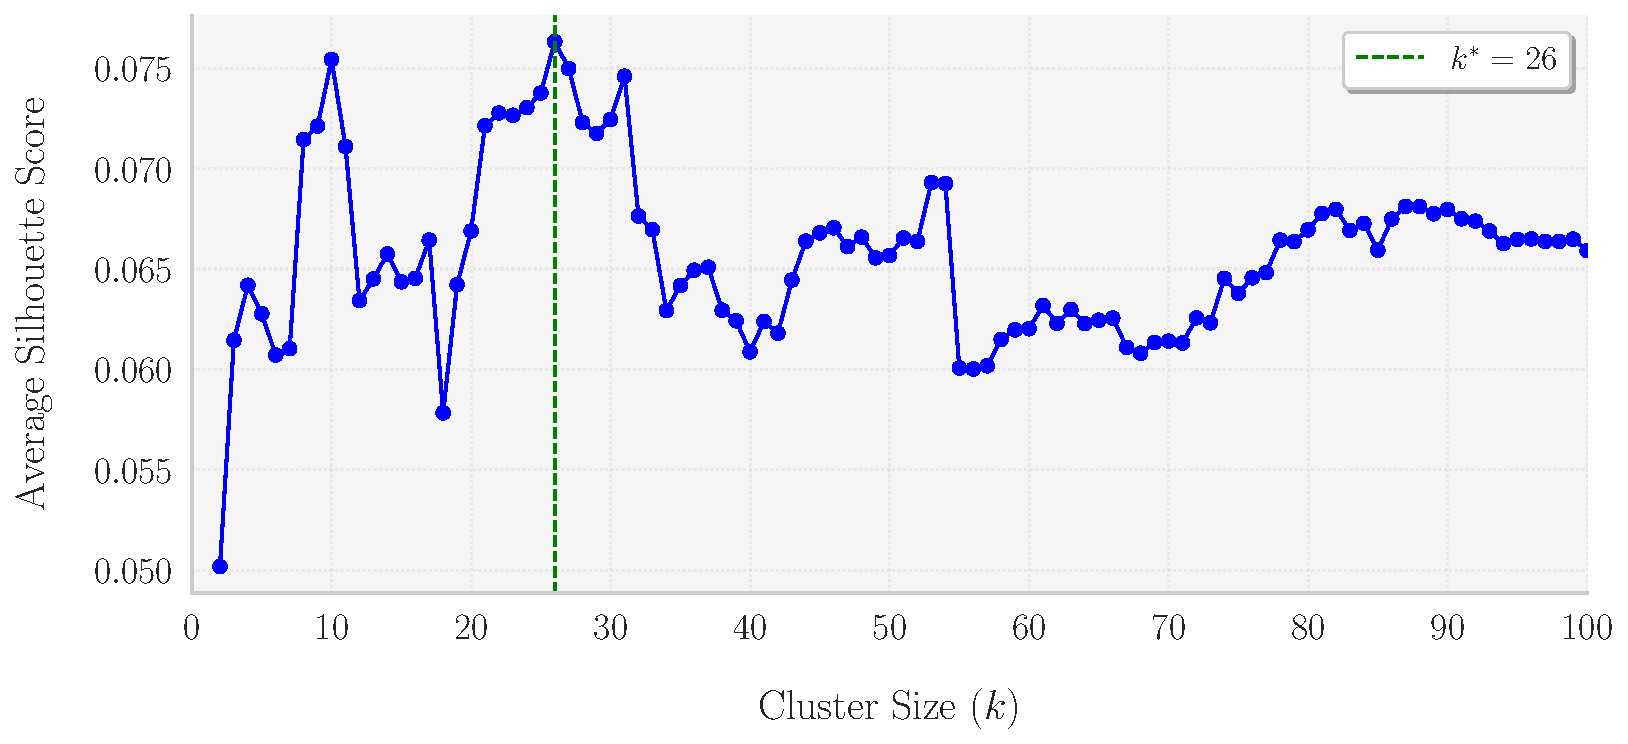
\includegraphics[scale=0.65]{/Users/jesusvillotamiranda/Library/CloudStorage/OneDrive-UniversidaddeLaRioja/CEMFI/__MSc__/__Second_year__/6th_Term/MasterThesis/__Output/KMeans_Clustering_Silhouette_Score.pdf}
%\subcaption*{\textit{Note: This plot shows the average silhouette scores computed on $\D^{tr}$ over a grid of possible cluster sizes $\mbf k=\{2,...,100\}$. The maximizer $k^*=26$ is highlighted with a vertical dashed green line.}}
\subcaption*{\textit{Note: The plot presents the average silhouette scores calculated on the training data $\D^{tr}$ for various cluster sizes $k$ ranging from 2 to 100. The silhouette score measures how well data points fit within their assigned cluster by comparing intra-cluster cohesion with inter-cluster separation. A higher silhouette score (closer to +1) indicates better-defined clusters. The optimal number of clusters, $k^*=26$, which maximizes the average silhouette score, is marked by a vertical dashed green line.}}
\label{fig:silhouette_score}
\end{figure}
%----------------------------------------------------




\mx
Given the optimal number of clusters $k^*$, we fit the KMeans algorithm on the training embeddings 
$\{\mbf e^i \mid i\in\D^{tr}\}$
%$\{ \mathbf{e}^1, \mathbf{e}^2, \ldots, \mathbf{e}^{N_{tr}} \}$
 to obtain the centroids $\{ \mathbf{c}^{tr}_1, \mathbf{c}^{tr}_2, \ldots, \mathbf{c}^{tr}_{k^*} \}$. Following \cref{alg:KMeans} (detailed in section A1 of the Appendix):
$$
\{ \mathbf{c}^{tr}_1, \mathbf{c}^{tr}_2, \ldots, \mathbf{c}^{tr}_{k^*} \} = \text{KMeans} ( \{ \mathbf{e}^1, \mathbf{e}^2, \ldots, \mathbf{e}^{N_{tr}} \}, k^* )
~.
$$

We then find the cluster associated to each embedding $\mathbf{e}^i$ in the validation set 
$\{\mbf e^i \mid i\in\D^{val}\}$ according to the centroids resulting from clustering the training data $\{\mbf c_1^{tr},..., \mbf c_{k^*}^{tr}\}$.
%$\{ \mathbf{e}^{N_{tr}+1}, \mathbf{e}^{N_{tr}+2}, \ldots, \mathbf{e}^{N_{tr}+N_{val}} \}$ to the nearest centroid $\mathbf{c}_g$. 
This allows us to obtain the clustering of the news articles in the validation sample
$$
\D_g^{val} = 
\3{ 
i\in \D^{val} 
\c g = \arg \min_{\ell\in\G} \|\mathbf{e}^i - \mathbf{c}^{tr}_{\ell}\|_{2}^2
}
\quad 
\forall g\in\G_{\t{KMeans}}
.
$$

Similarly, by assigning each embedding $\mathbf{e}^i\in \{\mbf e^i \mid i\in\D^{test}\}$
 to the nearest centroid $\mathbf{c}^{tr}_g$, we obtain the clusters in the test set
$$
\D_g^{test} = 
\3{ 
i\in \D^{test}
\c g = \arg \min_{\ell\in\G} \|\mathbf{e}^i - \mathbf{c}^{tr}_{\ell}\|_{2}^2 
}
\quad 
\forall g\in\G_{\t{KMeans}}
.
$$
%----------------------------------------------------

%
%%----------------------------------------------------
%\begin{figure}[H]
%  \centering
%  \caption{Distribution of articles through KMeans clusters}
%  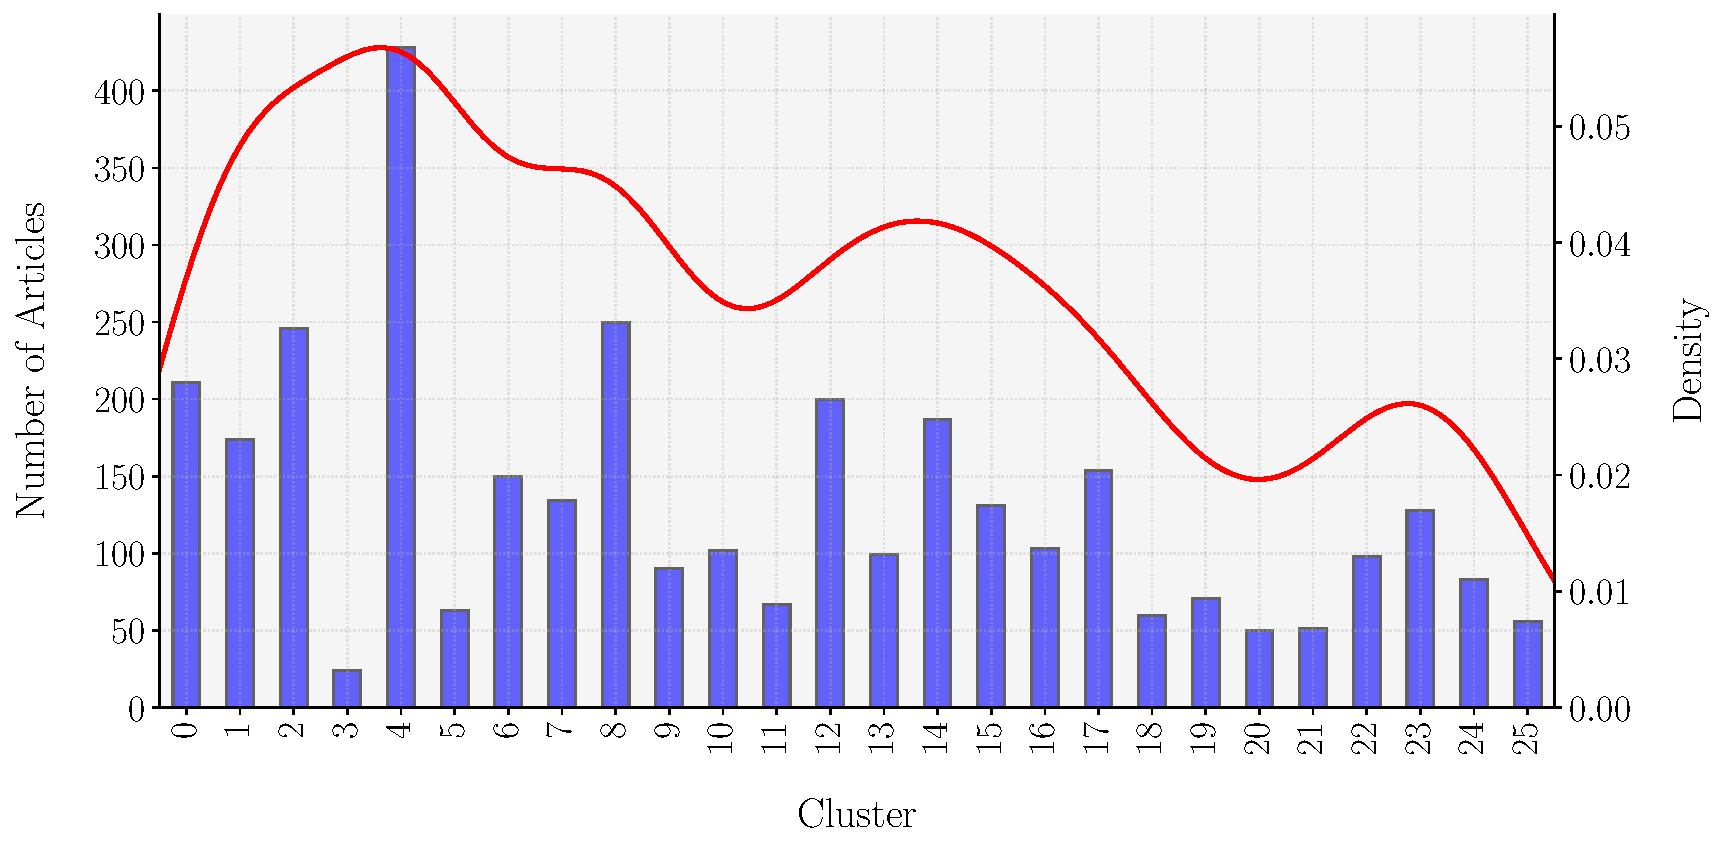
\includegraphics[scale=0.6]{/Users/jesusvillotamiranda/Library/CloudStorage/OneDrive-UniversidaddeLaRioja/CEMFI/__MSc__/__Second_year__/6th_Term/MasterThesis/__Output/KMeans_Cluster_Distribution.pdf}
%%  \caption{}
%\end{figure}
%%----------------------------------------------------
%
%
%%----------------------------------------------------
%\begin{figure}[h!]
%    \centering
%%    \caption{Distribution of articles through KMeans clusters across data splits}
%    \begin{subfigure}[b]{0.32\textwidth}
%        \centering
%        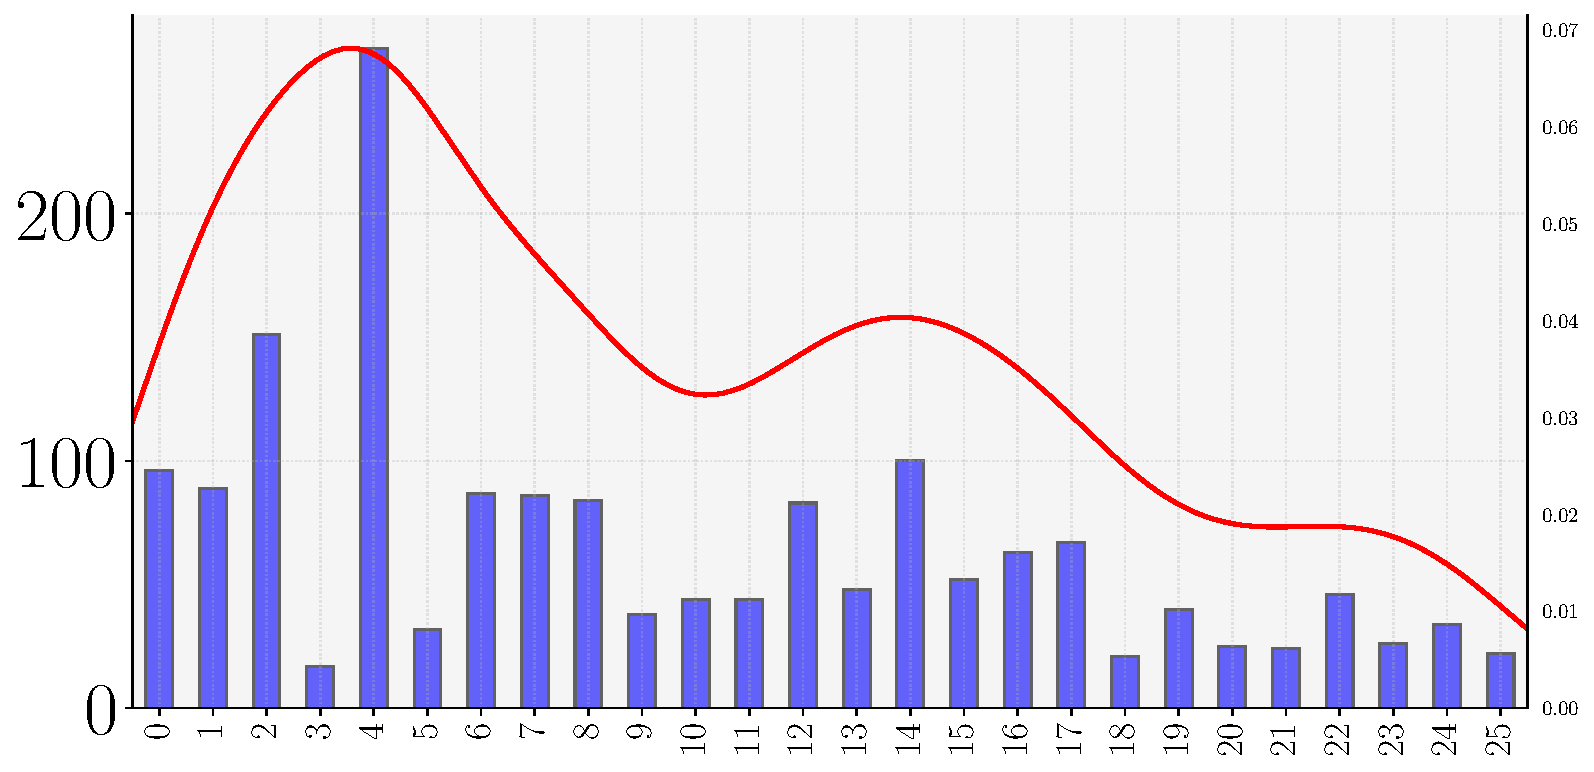
\includegraphics[width=\textwidth]{/Users/jesusvillotamiranda/Library/CloudStorage/OneDrive-UniversidaddeLaRioja/CEMFI/__MSc__/__Second_year__/6th_Term/MasterThesis/__Output/KMeans_Cluster_Distribution_Train.pdf}
%        \caption{Training data ($D^{tr}$)}
%        \label{fig:plot1}
%    \end{subfigure}
%    \begin{subfigure}[b]{0.32\textwidth}
%        \centering
%        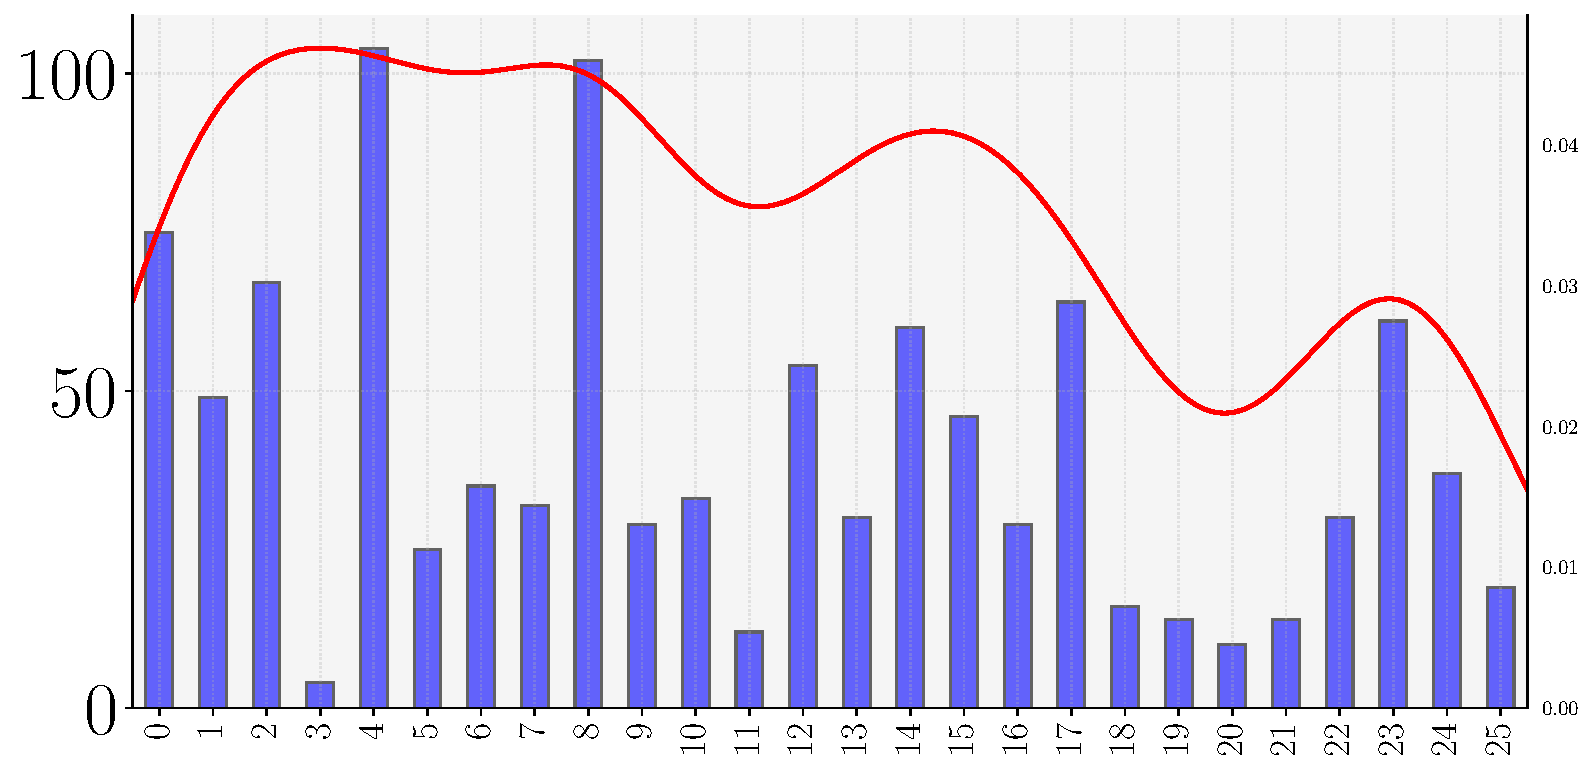
\includegraphics[width=\textwidth]{/Users/jesusvillotamiranda/Library/CloudStorage/OneDrive-UniversidaddeLaRioja/CEMFI/__MSc__/__Second_year__/6th_Term/MasterThesis/__Output/KMeans_Cluster_Distribution_Validation.pdf}
%        \caption{Validation data ($D^{val}$)}
%        \label{fig:plot2}
%    \end{subfigure}
%    \begin{subfigure}[b]{0.32\textwidth}
%        \centering
%        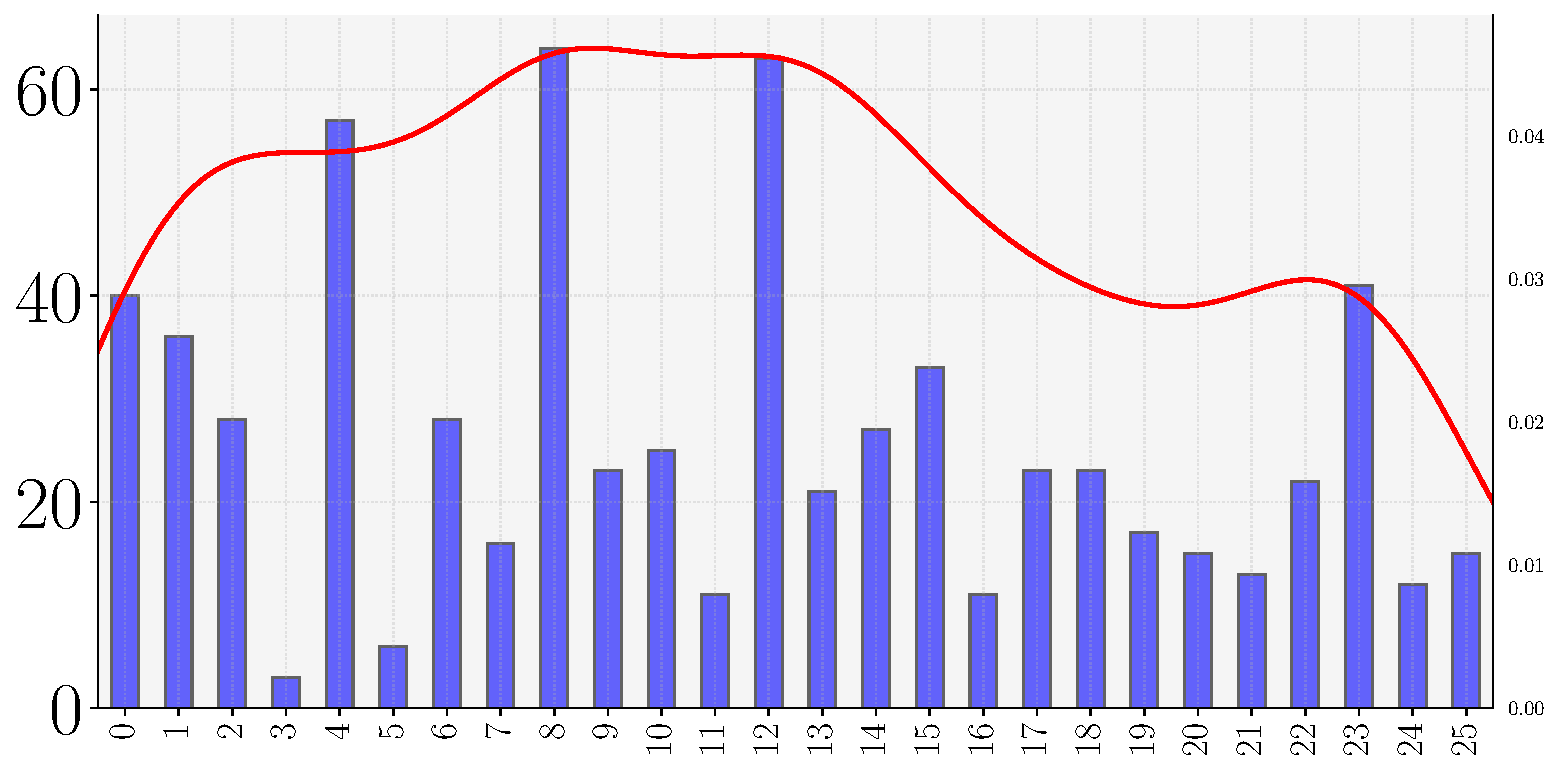
\includegraphics[width=\textwidth]{/Users/jesusvillotamiranda/Library/CloudStorage/OneDrive-UniversidaddeLaRioja/CEMFI/__MSc__/__Second_year__/6th_Term/MasterThesis/__Output/KMeans_Cluster_Distribution_Test.pdf}
%        \caption{Test data ($D^{test}$)}
%        \label{fig:plot3}
%    \end{subfigure}
%    \label{fig:three_plots}
%\end{figure}
%%----------------------------------------------------

%----------------------------------------------------
\inserthere{fig:combined_plots}
\begin{figure}[H]
    \centering
    \caption{Distribution of articles through KMeans clusters}
    
    % Upper plot
    \begin{subfigure}[b]{\textwidth}
        \caption{All data ($\mathcal D$)}
        \centering
        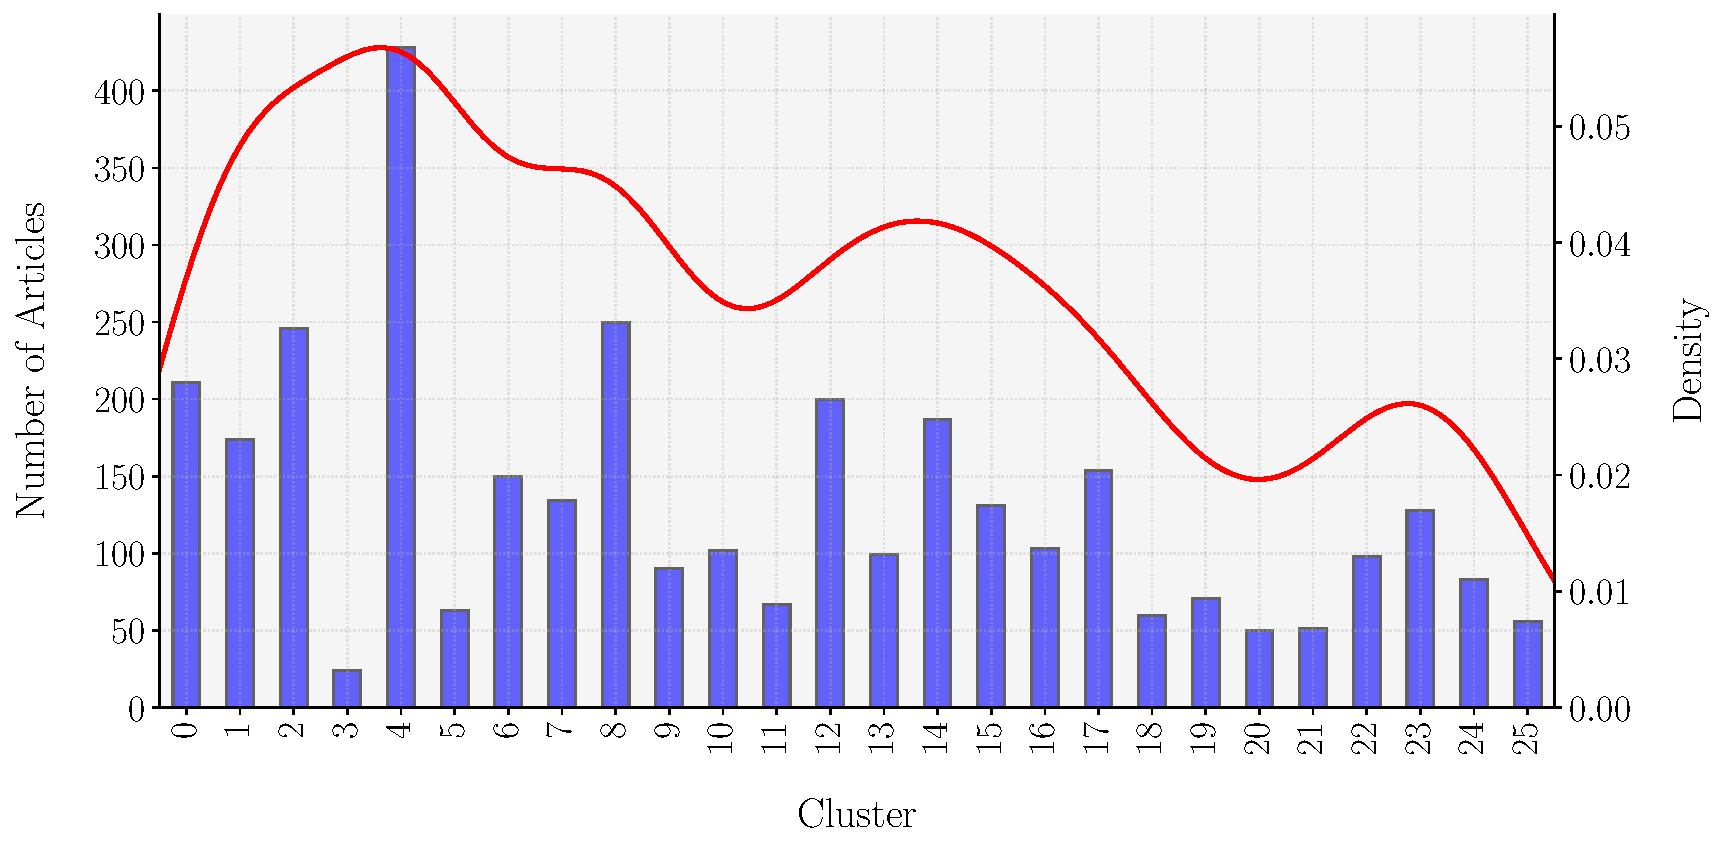
\includegraphics[scale=0.45]{/Users/jesusvillotamiranda/Library/CloudStorage/OneDrive-UniversidaddeLaRioja/CEMFI/__MSc__/__Second_year__/6th_Term/MasterThesis/__Output/KMeans_Cluster_Distribution.pdf}
        \label{fig:all_data}
    \end{subfigure}

    % Lower plots
    \begin{subfigure}[b]{0.32\textwidth}
        \caption{Training data ($\D^{tr}$)}
        \centering
        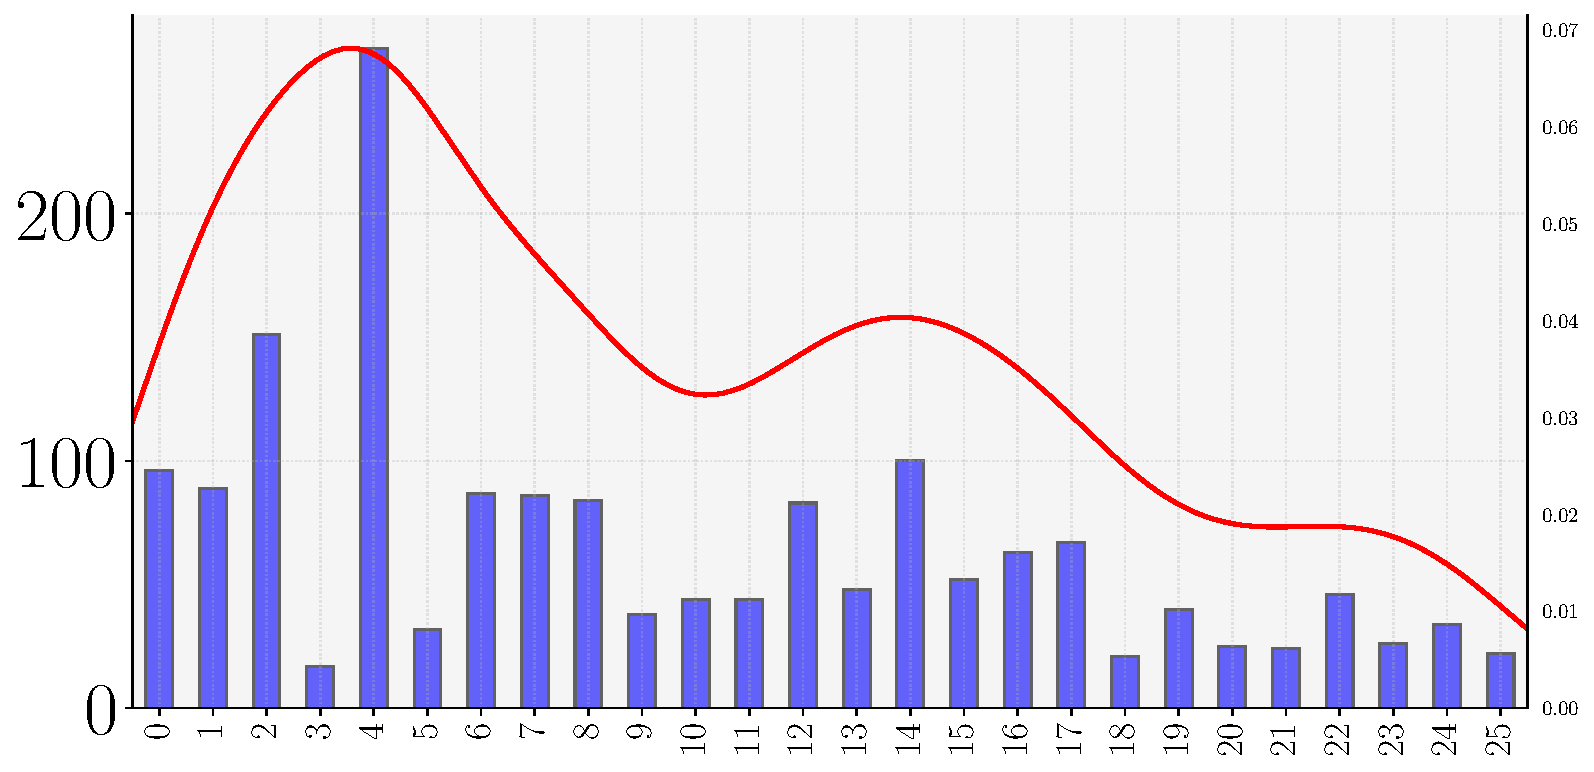
\includegraphics[width=\textwidth]{/Users/jesusvillotamiranda/Library/CloudStorage/OneDrive-UniversidaddeLaRioja/CEMFI/__MSc__/__Second_year__/6th_Term/MasterThesis/__Output/KMeans_Cluster_Distribution_Train.pdf}
        \label{fig:train_data}
    \end{subfigure}
    \begin{subfigure}[b]{0.32\textwidth}
        \caption{Validation data ($\D^{val}$)}
        \centering
        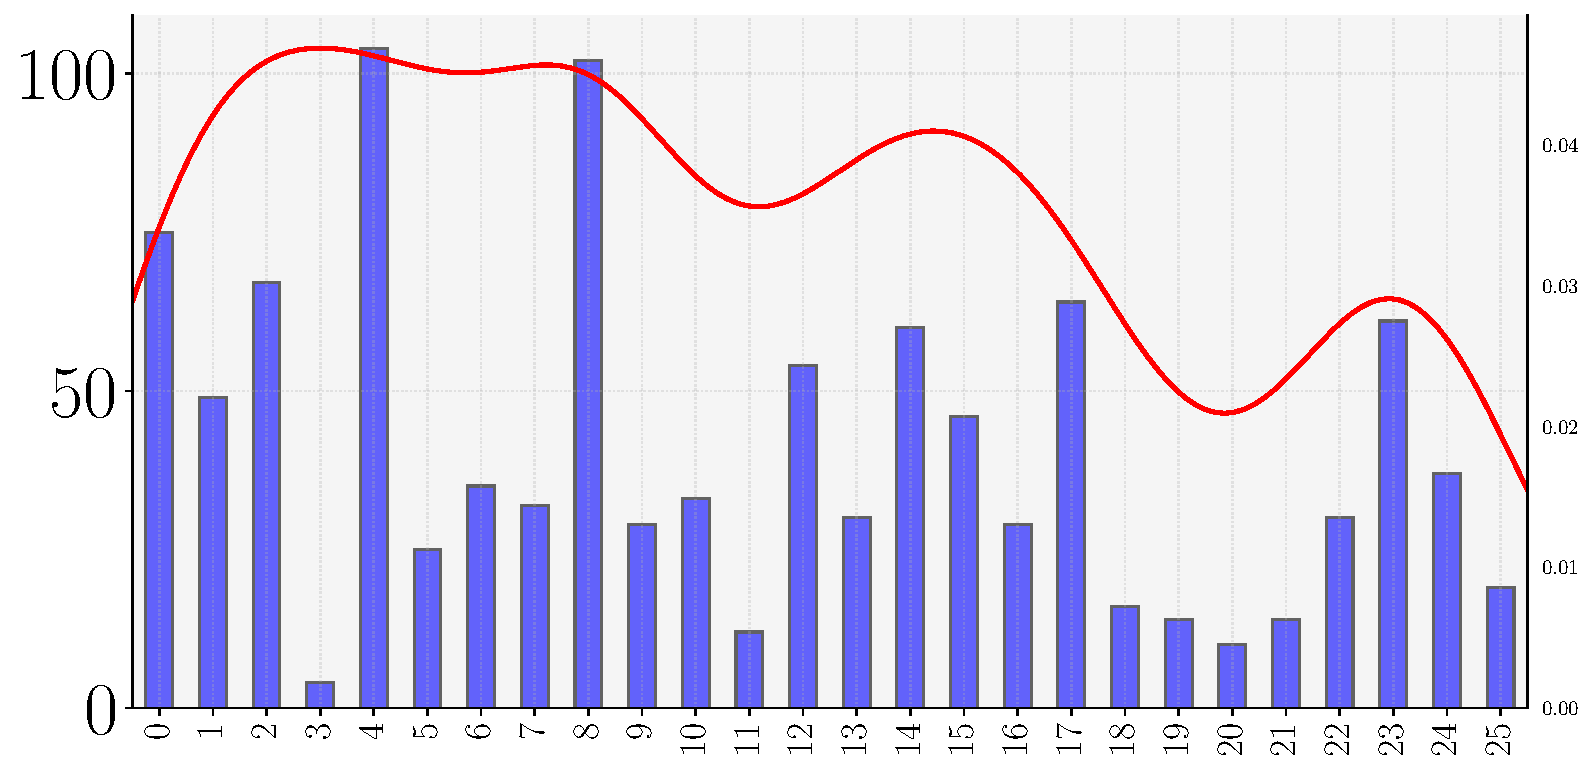
\includegraphics[width=\textwidth]{/Users/jesusvillotamiranda/Library/CloudStorage/OneDrive-UniversidaddeLaRioja/CEMFI/__MSc__/__Second_year__/6th_Term/MasterThesis/__Output/KMeans_Cluster_Distribution_Validation.pdf}
        \label{fig:val_data}
    \end{subfigure}
    \begin{subfigure}[b]{0.32\textwidth}
        \caption{Test data ($\D^{test}$)}
        \centering
        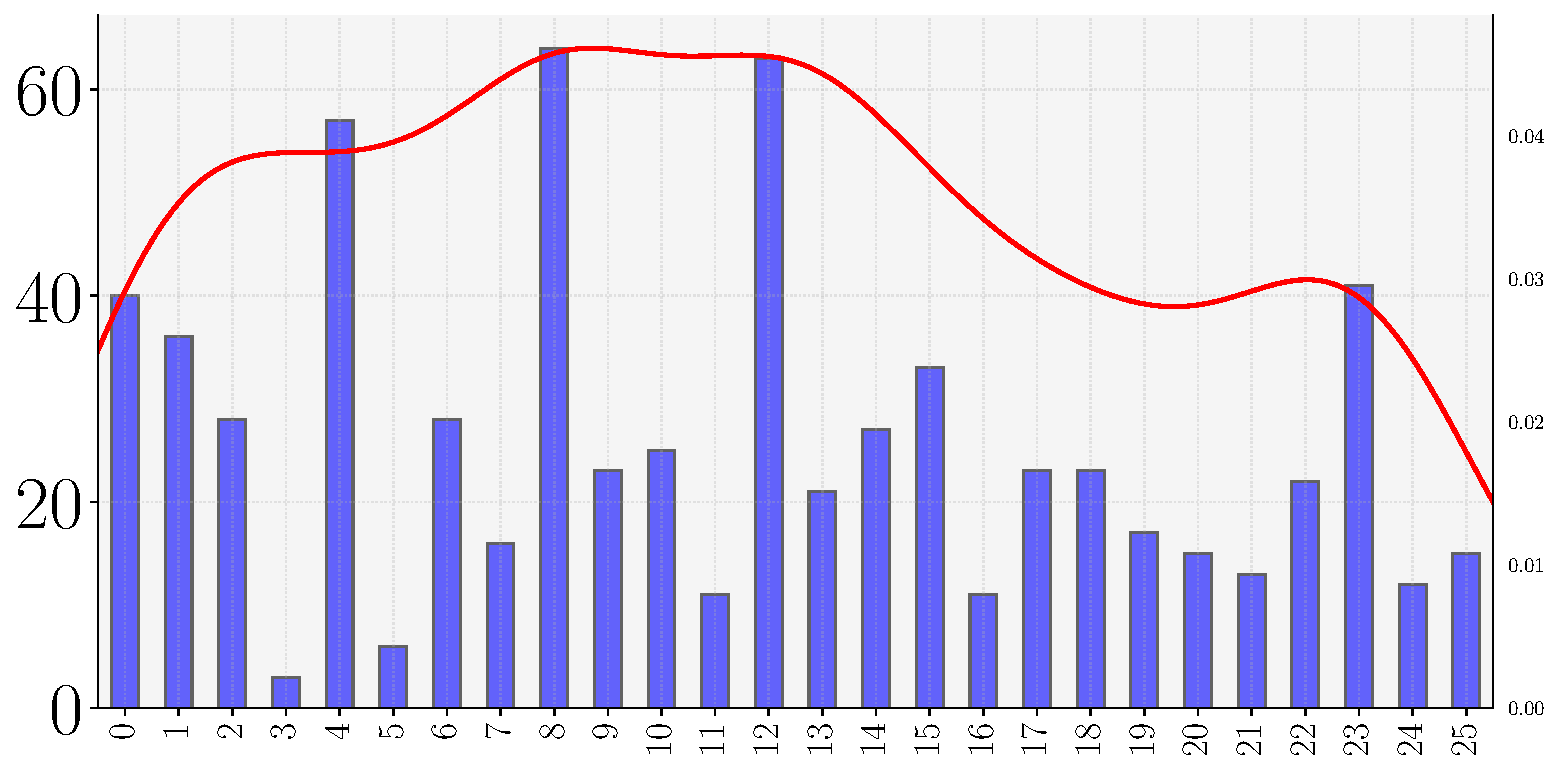
\includegraphics[width=\textwidth]{/Users/jesusvillotamiranda/Library/CloudStorage/OneDrive-UniversidaddeLaRioja/CEMFI/__MSc__/__Second_year__/6th_Term/MasterThesis/__Output/KMeans_Cluster_Distribution_Test.pdf}
        \label{fig:test_data}
    \end{subfigure}
    \label{fig:combined_plots}
%\subcaption*{\textit{Note: The upper plot shows the distribution of articles $i\in \mathcal D$ through clusters found by applying KMeans to $\mathcal D$. The lower plots show the distributions of articles through clusters for the training ($\D^{tr}$), validation ($\D^{val}$), and test ($\D^{test}$) articles through clusters .}}
%\subcaption*{\textit{Note: This figure shows the distribution of articles through each of the $k^*=26$ clusters. The centroids of such clusters come from applying KMeans to the vector embeddings of the articles in the training data. Panel A shows the overall distribution for the whole data ($\mathcal D$), while Panel B, C and D show the split-specific distributions, respectively, for training ($\mathcal D^{tr}$), validation ($\mathcal D^{val}$) and test data ($\mathcal D^{test}$).
%}}
\subcaption*{\textit{Note: This figure presents the distribution of articles across the $k^*=26$ clusters, where the centroids were determined by applying the KMeans algorithm to the article embeddings from the training data. Panel \textsc{(a)} shows the distribution for the entire dataset ($\mathcal{D}$), while Panels \textsc{(b)}, \textsc{(c)}, and \textsc{(d)} illustrate the distributions for the training ($\mathcal{D}^{tr}$), validation ($\mathcal{D}^{val}$), and test ($\mathcal{D}^{test}$) datasets, respectively. The differences in distribution across splits suggest some temporal instability in the clustering results.}}
\end{figure}
%----------------------------------------------------

As we can see, the distribution of articles in the whole sample ($\D$) is fairly homogenous across the 26 clusters, with each cluster containing between 50 and 250 articles on average. The notable exceptions are cluster 3, which contains only 24 articles, and cluster 4, which concentrates 428 articles. However, the distribution profile is not consistent over data splits, which indicates that this classification procedure is unstable over time.

\mx 
Although not directly interpretable, by looking at the articles pooled in a certain cluster, we can provide some intuition of what it represents. In most cases, each cluster contains articles involving a firm or set of firms in the same sector. For example, cluster 3 pools articles about Telef�nica and Cellnex (telecoms), cluster 4 contains articles about CaixaBank, cluster 9 concentrates articles about Repsol, cluster 12 about Iberdrola, cluster 15 gathers articles on Infrastructure (led by ACS and Acciona) and so on.

\mx 
However, there are some exceptions to this general rule, for example, cluster 0 is a \qquote{miscellanous} cluster:
% with no clear pattern: 
 it covers articles about different firms with no apparent relation between them. Another example is cluster 1, which pools articles related to the quarterly or semiannual publication of results by different firms. In \cref{tab:KMeans_Articles_3_English} of the Appendix we provide a sample of 3 articles for each cluster and propose a name for each one based on the articles they pool.
